\chapter{Etats de l'art}
\label{ch:state_art}

\section{introduction}
Dans ce chapitre nous aborderons les différentes pistes envisagées afin de remplir les objectifs fixés dans cette thèse, comme listé dans l'introduction (\cf{ch:introduction}).

Avant toutes choses il à fallu se mettre au niveau et comprendre la thèse \thLeite.

\section{Automatisation}
En terme d'automatisation, une pratique bien courante chez les developpeur s'agit à utiliser des script bash afin de pouvoir executer une certain nombre de commande et de code succecivement. Bien que cette méthode présente l'avantage d'etres simple, il suffit d'une console UNIX et d'un editeur de texte, elle présente un défault majeur. En effet, le developpeur du script contrôle quel commande et code sont executé et peut également definir des paramètres pour ceux-ci, mais il ne peu pas contrôlé l'environnement d'execution.

Une façcon de faire, en pleine essort depuis quelque temps, est l'utilisation de la platforme Docker. Il s'agit d'un logiciel de containerisation. C'est-à-dire la création de brique d'application qui mise en communes permette de réaliser un application global. De plus, le développement d'une telle solution, permet un partage facilité grâce à un déploiement facilité et autonome. Pour d'avantages d'explication sur le sujet je vous renvoi au chapitre  \cf{ch:docker}.

Vous l'aurez bien compris, le choix qui à été fait est celui de l'utilisation de Docker.

\section{Configuration}

En ce qui concerne la recherche d'une méthode afin de réalisé facilement des fichiers de configurations pré-créées, beaucoup de solutions existent. Ces différentes méthodes sont plus ou moins flexible aux modifications.

Les fichiers de configurations dont il est question ici, sont spécifique à la partie python du code qui sera executé par notre application \cf{ch:app}. En effet, l'on souhaite entre autre être capable de donner des fichiers de configuration en entrée et d'obtenir pour chacuns un résultats en sortie.

Nous ne citerons ici uniquement la solution retenu, car les autres solutions trouvée sont soit trop incompatible soit presque identique à la solution retenu.

Nous utilisons le module python \emph{Configparser}, qui permet de lire et parser des fichiers à l'extension .ini de manière simple. De plus, la structure d'un fichier .ini est très simple et ne laisse donc que très peu de place aux erreurs de format.
 
 
\section{Hmmer}
%Hmmer
Dans la thèse \thLeite les séquences protéiniques sont recherché dans la base de données de profile-HMM à l'aide d'une \gls{api} en ligne. Cette \gls{api} est disponible depuis le site \emph{https://www.ebi.ac.uk/Tools/hmmer/}. 

Comme dis précédement, un de objectifs de ce travail est de se passer de l'utilisation de cette \gls{api} car sont accès n'est pas toujours disponible ou stable.

Une recherche rapide à permis de se rendre compte que l'application utilisé derrière cette \gls{api} est disponible au téléchergement et peut donc etres utilisée de manière local. Pour d'avantage d'information \cf{ch:app}, sous-chapitre Hmmer.


\section{Parallélisation}

La version existante du code se trouvant dans la thèse \thLeite est une version sous forme de scrit, proof-of-concept, en python2 et non \emph{multiprocessed}. Afin de garantir une utilisation optimal des ressources de la machine hote, sur laquelle le code est executé, nous souhaitons rendre le code parallèle là où il est possible de le faire.

Plusieures solution sont possible, encore une fois les solutions les plus compliquées ne sont pas toujours celle les plus efficaces. De plus une méthode trop complexe pourrait réduire la bonne transmition du code à d'autre développeurs.

La partie principal que l'on souhaite paralleliser est l'utilisation de la fonction de scanne de HMMMER, étant donné qu'un très grand nombre de séquences protéinique doivent être analysées.

\subsection{Simple}
\subsubsection{Docker}
Docker, mise à part de rendre le déploiement et l'execution d'application automatisée, parmet également de lancer plusieurs containers simultanéement, \cf{ch:docker}. Un container englobe un systeme de fichier complete possèdant tous se qu'y est necessaire a remplir sa fonction. 

\subsubsection{Python}
En python on retrouve deux principal méthode permettant de réaliser de code parallel. En effet, on peut utiliser le \emph{multiprocessing} ou le \emph{multithreading}.

Notre bute est de réaliser et d'optimiser un code \gls{cpu} dépendant, c'est-à-dire coeurs dépendant. Lors de l'utilisation du langage python il faut savoir qu'avec des code \gls{cpu} dépendant, python limite les possibilité de parallelisme à cause de la \gls{gli}. La \gls{gli} est necessaire en python, car python n'est pas \emph{tread safe}. En effet, il y a, en python, un verrou global lorsque l'on essaye d'acceder a un objet depuis un thread.

A cause de se verrous les codes \gls{cpu} dépendant ne gagnerons pas en pérformance lorsqu'ils sont parallélisé à l'aide de \emph{multithreading}, mais uniquement avec le \emph{multiprocessing}.

\subsection{Avancée}
\subsubsection{Docker Swarm}
Une autre méthode utilisant une librairie avancé de Docker, consiste à utiliser Docker Swarm. Docker Swarm apporte à DOcker une gestion native du \emph{clustering}, afin de transformer un groupe de \emph{Docker engines} en un unique et virtuel \emph{Docker engine}. Grâce à cela il est possible d'executer une application sur un architecture partagée sur plusieurs système physiquement indépendant. 

\subsubsection{Spark}
Spark est un framework \emph{open source} de calcule distribué. Il permet d'effectuer des analyse complexes sur un grand nombre de données.

Il est également un ensemble d'outils pour le traitemnt de grandes source de données, notament grace à des fonctions \emph{MapReduce}.
	
\section{Optimisations}
Le code repris de la thèse \thLeite est un code séquetielle, sous forme de script necessitant des input utilisateurs a chaque étapes. De plus ce code est ecrit en python dans sa version 2.

Grâce au travail du Dr. Brett Cannon, \href{https://speakerdeck.com/pyconslides/python-3-dot-3-trust-me-its-better-than-python-2-dot-7-by-dr-brett-cannon}{See here}, on se rend compte que python 3.3 pourrait optimiser les performance de notre application. On peu lire 
\href{https://mail.python.org/pipermail/python-dev/2012-October/121923.html}{ici} que même 'appel des fonctions est en moyenne 1.20 fois plus rapide. De plus, les \emph{threadded count} sont également plus rapide.

Une autre possibilité est d'utiliser \emph{Cython}. Cython est un compilateur/language de python permettant d'utiliser de appele au langague C et de compiler un code python en executable C. Il faut savoir qu'un executable C est généralement plus rapide que l'execution de l'interpreteur python. 

On trouve le tableau suivant dans la documentation de Cython, qui permet de nous rendre compte des différences.

\begin{figure}[H] 
\centering 
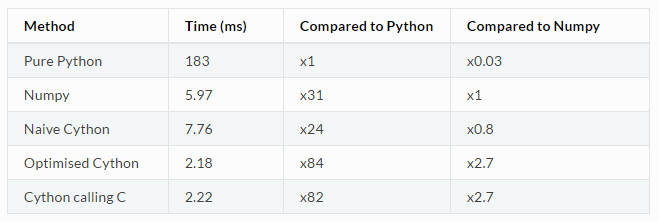
\includegraphics[width=1\columnwidth]{img/table_cython} 
\caption[Tableau performences Cython]{Tableau de comparaison de Cython - \url{http://notes-on-cython.readthedocs.io/en/latest/std_dev.html/}).}
\label{fig:galleria} 
\end{figure}

\section{conclusion}
Après des tests sur ces différente technologies et méthodes et quelques disscutions ici et là, l'idée ayant été arreté est d'utiliser \emph{Docker} et \emph{Docker Compose} comme contexte applicatif et de transformer les script en une application orientée objet en python 3.3 gérant les fichiers de configurations avec la librairie \emph{Configparser}. Pour ce qui est du parallélisme, il sera réalisé en utilisant la librairie \emph{Multiprocess}.
















